% A linear map T : V -> W sent basiswise; the top k basis vectors map
% to image vectors and the rest to 0, exhibiting ker T and im T.
% Source: book/tex/linalg/vector-space.tex (§ What is a linear map intuitively?).
\documentclass[border=2mm]{standalone}
\usepackage{tikz}
\usepackage{amsmath,amssymb}
\usetikzlibrary{arrows.meta}
\begin{document}
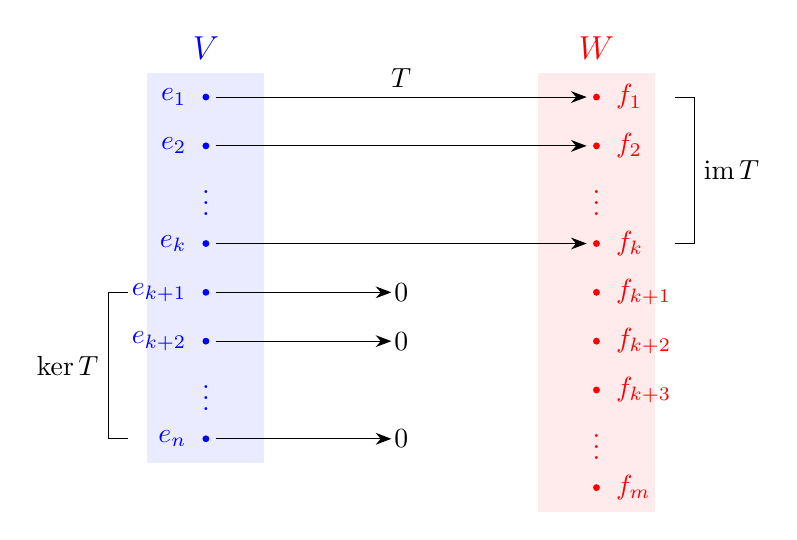
\begin{tikzpicture}[scale=0.62,>={Stealth[length=2mm]}]
  \fill[blue!8] (-5.2,3.5) rectangle (-2.8,-4.5);
  \fill[red!8]  (2.8,3.5) rectangle (5.2,-5.5);
  \node[blue] at (-4,4) {\large $V$};
  \node[red]  at (4,4)  {\large $W$};
  % V basis
  \foreach \y/\lab in {3/e_1,2/e_2,0/e_k,-1/e_{k+1},-2/e_{k+2},-4/e_n}
    {\fill[blue] (-4,\y) circle (2pt); \node[blue,left] at (-4.2,\y) {$\lab$};}
  \node[blue] at (-4,1) {$\vdots$}; \node[blue] at (-4,-3) {$\vdots$};
  % W basis
  \foreach \y/\lab in {3/f_1,2/f_2,0/f_k,-1/f_{k+1},-2/f_{k+2},-3/f_{k+3},-5/f_m}
    {\fill[red] (4,\y) circle (2pt); \node[red,right] at (4.2,\y) {$\lab$};}
  \node[red] at (4,1) {$\vdots$}; \node[red] at (4,-4) {$\vdots$};
  % T arrows (nonzero part)
  \foreach \y in {3,2,0} \draw[->] (-3.8,\y)--(3.8,\y);
  % zero part
  \foreach \y in {-1,-2,-4} {\draw[->] (-3.8,\y)--(-0.2,\y); \node at (0,\y) {$0$};}
  \node[above] at (0,3) {$T$};
  % im and ker brackets
  \draw (5.6,3)--(6,3)--(6,0)--(5.6,0); \node[right] at (6,1.5) {$\operatorname{im} T$};
  \draw (-5.6,-1)--(-6,-1)--(-6,-4)--(-5.6,-4); \node[left] at (-6,-2.5) {$\ker T$};
\end{tikzpicture}
\end{document}
